
\documentclass[12pt]{book}
\usepackage{cclicenses}
\usepackage[letterpaper,  hmargin = { 1in},vmargin = { 1in}]{geometry}
\usepackage{hyperref}
\usepackage[T1]{fontenc}
\usepackage{multicol}
\newcommand{\mytitle}{Scivault Physics}
\usepackage{amsmath}
\usepackage{mathtools}
\usepackage{enumitem}
\usepackage{cleveref}
\usepackage{longtable}
\usepackage{appendix}
\usepackage{makeidx}
\usepackage[makeroom]{cancel}
\usepackage{tikz}
\usepackage[linewidth=1pt]{mdframed}
\setlength{\columnsep}{1cm}

\makeindex

%%% To make index work,
% 1) Compile
%2) From base directory, run:
%   makeindex "Scivault Physics.idx"
%3) Compile again

\begin{document}
	\frontmatter
	\title{\mytitle}
	\author{Jonas Williamson}
	\date{Version \the\year\the\month\the\day}
	\maketitle

\normalsize
	\copyright \space \the\year\space by Jonas Williamson.  All Rights Reserved. 
	
		\vspace{2 in}	


	\vspace{1 in}

	\tableofcontents


\mainmatter


	
	
	
	
	
	

	
	


\chapter{Introduction}
\section{Dimensional Analysis and SI units}
The \textbf{SI}\index{SI system of units} system of units is the standard used by many scientists throughout the world.  There are seven \textit{fundamental} or \textit{base} quantities from which all other measurements are derived.  These quantities are listed below:
 \index{Units, Fundamental}

\begin{center}

	
\begin{table}[ht]\caption{\textbf{SI Units}}% title of Table 
	\centering % used for centering table	
	\begin{tabular}{|c|c|c|}
		\hline \hline
		\textbf{Quantity} & \textbf{Unit} & \textbf{Unit Symbol}\\
		\hline
		time & second & s \\
		\hline
		length & meter & m \\
		\hline
		mass & kilogram & kg \\
		\hline
		electrical current & Ampere & A \\
		\hline
		temperature & Kelvin & K \\
		\hline
		amount of substance & mole & mol \\
		\hline
		luminous intensity & candela & cd \\
		\hline		
	\end{tabular}
	\label{table:nonlin}% is used to refer this table in the text
\end{table}
\end{center}

	Of these quantities, mass, time and length are quite common.  Thus, this system is sometimes called the MKS (meter, kilogram, second) system. In order to use any equations, all measurements must have correct units.  For example, if a time is expressed in hours, it must first be converted into seconds before any calculations can be attempted.  
	
	Dimensional analysis \index{Dimensional Analysis} is the process in which the units associated with quantities create \textit{derived units}. \index{Units, Derived} For instance, when a distance is divided by a time, the units will be $ \frac{m}{s}$ (read \textit{meters per second}).  	
	
	Dimensional analysis is an important part of solving physics problems.  Often, correct dimensional analysis can help you determine if a problem has been solved correctly.  One should not even attempt to calculate an answer to a problem until the correct units have been verified. 



		


\section{Vectors and Scalars}
In the study of physics, there are two types of quantities that we will deal with on a regular basis: \textit{scalars} and \textit{vectors}.  

A \textbf{scalar} is a quantity that you are already most likely very familiar with, as it is just a number; scalars have only a \textit{magnitude} (a number that represents how big or strong it is), and can sometimes include units.  Examples of scalars might be the number of people in a room, the mass of a car, or your age in years.  

\textbf{Vectors} are different from scalars because in addition to a magnitude, they contain a direction as well.  Examples of vectors might include 50 feet to the north, 5 m/s at a 33$^\circ$ angle, or 200 miles straight up.  
There are many ways of expressing vectors.  Symbollically, they are often written with an arrow over them.  For example, in the equation \color{blue} $\vec{F} = m \vec{a}$ \color{black}  both force and acceleration are vectors – meaning that both force and acceleration have a direction.  Sometimes vectors will be expressed in \textbf{bold} typeface.   Hence, the expression \\ \color{blue} \textbf{F} = m \textbf{a}  \color{black} is equivalent to the expression shown above.

The direction for vectors in 1 dimension is easy – all you need is a positive or a negative.  Usually, 1-dimensional motion takes place along the x-axis (left and right), but sometimes it will take place in the y- (forward and backward) and z- (up and down) dimensions.  For the purposes of this book, positive is to the right and up unless otherwise stated. 
In two dimensions, a vector requires two pieces of information.  One way of expressing a vector is in polar form.  Polar form in two dimensions includes a magnitude of the vector and an angle, usually measured from the x-axis.  There are several ways for writing this.  4 cm @ 15$^\circ$, \\ 4 cm $\angle 15^\circ$ and 4 cm at 15$^\circ$ North of East all represent the following displacement vector:
	\begin{center}
		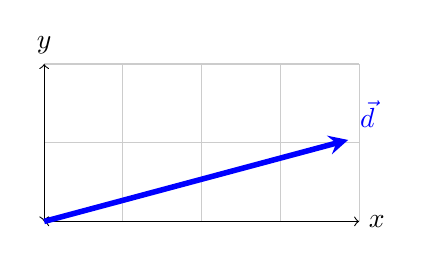
\begin{tikzpicture}
		\draw[thin,gray!40] (0,0) grid (4,2);
		\draw[<->] (0,0)--(4,0) node[right]{$x$};
		\draw[<->] (0,0)--(0,2) node[above]{$y$};
		\draw[line width=2pt,blue,-stealth](0,0)--(3.86,1.035) node[anchor=south west]{$\vec{d}$};
	
		\end{tikzpicture}
	
	
	
	\end{center}

	
	Unit vectors are vectors that have a length of one unit and are oriented along one axis.  The unit vector for the x-direction is written as $\hat{i}$ (pronounced i-hat).  $\hat{i}$ is a 1-unit long vector that is always parallel to the x-axis, and points in the direction of increasing x values.  Likewise, the y-direction and z-direction unit vectors are written as $\hat{j}$ and $\hat{k}$ respectively.  
	
	
	Because the surface of a paper is effectively 2-dimensional, it is very hard to draw lines that are oriented directly into or out of your paper. For this purpose, physicists have agreed to the following convention: vectors that point directly into your paper are notated by $\bigotimes$ .  Vectors that point directly out of your paper are shown by the symbol $\bigodot$.  
	
	Sometimes, vectors may be expressed in Cartesian coordinates.  This vector could either be expressed as an ordered pair (or triple) with square brackets, such as [3, 4, 5] cm, or as a linear combination of the unit vectors shown above, such as $5\hat{i} + 12 \hat{j} + 3 \hat{k}$  In each case, the distances in each direction are given by the numbers shown.
	
	When converting between polar and cartesian forms for two dimensional vectors, a little trigonometry shows: 
	\color{blue}
	\begin{multicols}{2}
		\begin{center}
			\begin{equation}
			x = r \cos(\theta)
			\end{equation}
			
			\begin{equation}
			y = r \sin(\theta)
			\end{equation}

			\begin{equation}
			r = \sqrt{x^2+y^2}			
			\end{equation}

			\begin{equation}
			\theta=\tan^{-1}(\frac{y}{x})
			\end{equation}		
		\end{center}
	\end{multicols}
	\color{black}
	In three dimensions, polar form comes in two types – Cylindrical and Spherical.  In cylindrical coordinates, expressed as [r, $\theta$, z],  the above conversions are used, and the z-coordinate remains unchanged from Cartesian form.  We will study spherical coordinates more in \color{red} INSERT REFERNCE HERE! \color{black}
	
	
	
	
	
\section{Vector Mathematics}
	\subsection{Vector Addition}
	\subsection{The Dot Product}
	\subsection{The Cross Product}
	

\chapter{Kinematics in One Dimension}
\section{Distance and Displacement}
You are probably already familiar with the concept of \textbf{distance} – you might get in your car and drive a total of 1.2 miles to school, turning right after 0.45 miles, according to your car's odometer.  Distance is a scalar that tells you how far something traveled.  d usually represents distance.

While you may have traveled a total distance of 1.2 miles from your school, you are significantly less than 1.2 miles away from home; in fact, you are approximately 0.874 miles from home, following a direct path directly from your home to the school, at an angle of $59^\circ $(not worrying that this path might take you through someone's back yard or kitchen).  \textbf{Displacement} is a vector that tell you how far something is from the origin, and is independent of the path taken to get there.  The displacement vector is commonly symbolized by $\vec{r}$ though sometimes it may be written as $\vec{d}$. 

\section{Average and Instantaneous Speed and Velocity}

\textbf{Speed} is a scalar value that represents the change in distance per change in time of an object.  Speed is usually represented with the symbol $v$, without the vector sign.  You are probably already familiar with this quantity, since the speedometer on your family car measures speed.  For the purposes of physics, speed has little value because it is a scalar that tells us nothing of direction.  Much more useful is the concept called velocity.  Velocity and speed are related much like distance and displacement.  

\textbf{Velocity} is the change in displacement of an object per unit time, and as such is a vector.  Positive velocities indicate that the object is moving forward, relative to the axis in question, and negative velocities generally mean that the object is moving backward, relative the the axis.  The average velocity of an object is given by:
\begin{center}
	\begin{equation}
	\overrightarrow{v_{avg}} = \frac{\Delta\vec{r}}{\Delta t}
	\end{equation}
\end{center}

Average velocity is useful if an object's velocity is not changing.  However, many times it is more useful to talk about instantaneous velocity.  Instantaneous velocity tells us how fast an object is moving at a given instant in time.  In order to calculate instantaneous velocity, we must allow our time interval in the above formula to become infinitesimally small.  In this case, a little calculus proves:

	\begin{equation}
	\vec{v} = \frac{d\vec{r}}{dt}
	\end{equation}
	
	
	Calculation of average velocity is rather straightforward, assuming you know both distance traveled and the time it took.  If an object is not speeding up or slowing down during a specific time interval, the instantaneous velocity at any time during this interval is equal to the average velocity.  If the object does speed up or slow down during the time interval in question, the average velocity and the instantaneous velocity at a certain time during the interval are not necessarily the same. 
	
\begin{mdframed}[backgroundcolor=blue!10!white]
		\begin{center}


		\textbf{Example \thesection.1}	
	\end{center}

You ride your bicycle in a straight line for a distance of 73 meters in 12.5 second.  What is your average velocity?

Solution:
\begin{equation}
 a
\end{equation}

\end{mdframed}
	

\section{Relative Motion at Constant Velocity}
\section{Acceleration}
\section{The Kinematic Equations}
\section{Vertical Motion and Gravity}



\chapter{Graphing Motion}
	\section{Position vs Time Graphs}
		\subsection{Constant Position}
		\subsection{Constant Velocity}
		\subsection{Constant Acceleration}
	\section{Velocity vs Time Graphs}
		\subsection{Constant Position}
		\subsection{Constant Velocity}
		\subsection{Constant Acceleration}
	\section{Acceleration vs Time Graphs}
		\subsection{Constant Position}
		\subsection{Constant Velocity}
		\subsection{Constant Acceleration}	
	

	



\chapter{Kinematics in Two Dimensions}
	\section{Introduction}
	
	When an object is moving in two (or three) dimensions at once - like when it moves both horizontally and vertically at the same time - the motion of the object in each dimension is completely independent.  This means that each dimension will have its own set of kinematic variables.  The only kinematic variable that can be used in all directions is time, since time is a scalar and does not have a direction.  Thus, instead of only five kinematic variables, problems will have sets of five variables in each direction, with time counting for every dimension.  
	
	
{\renewcommand{\arraystretch}{1.2}
\begin{center}
	
	
	\begin{table}[ht]\caption{\textbf{Kinematic Variables in Multiple Dimensions}}% title of Table 
		\centering % used for centering table	
		\begin{tabular}{|c|c||c|c|}
			\hline \hline
			\textbf{Quantity} & \textbf{Variable} & \textbf{Quantity} & \textbf{Variable}  \\
			\hline
			Horizontal Displacement & $\vec{d_x}$ or $\vec{x}-\vec{x_0}$  & Vertical Displacement & $\vec{d_y}$ or $\vec{y}-\vec{y_0}$ \\
			\hline
		
			Horizontal Initial Velocity & $\vec{v_{ix}}$ or $\vec{v_{0x}}$  & Vertical Initial Velocity & $\vec{v_{iy}}$ or $\vec{v_{0y}}$ \\
\hline

			Horizontal Final Velocity & $\vec{v_{fx}}$ or $\vec{v_x}$  & Vertical Final Velocity & $ \vec{v_{fy}}$ or $\vec{v_y}$ \\ 
	\hline
	Horizontal Acceleration & $\vec{a_x}$  &  Vertical Acceleration & $\vec{a_y} $ \\
	\hline
	\multicolumn{2}{|c|}{Time} & \multicolumn{2}{|c|}{$t$} \\
	\hline
		
		\end{tabular}
		\label{table:kinematic2d}% is used to refer this table in the text
	\end{table}
\end{center}

\section{Projectiles}
\index{Projectiles}

A \textbf{projectile} is any object that meets the following critera:
\begin{itemize}
	\item The object is in \textit{free-fall}.  That is, Gravity is the only force that acts on the object (all other forces are negligable).
	\item The object is moving in two dimensions at the same time.  Most often, describe it as moving both horizontally and vertically at the same time.  
\end{itemize}


\subsection{Horizontally Launched Projectiles}
	\index{Projectiles, Launched Horizontally}
Often, projectiles will be launched horizontally, such as when a ball rolls off a table, or when an archer shoots a perfectly level arrow.  In this case, the math is somewhat easier to deal with.  The initial velocity stated in the problem will be entirely horizontal, and the initial vertical velocity will be zero.


\begin{mdframed}[backgroundcolor=blue!10!white]
	\begin{center}
		
		
		\textbf{Example \thesection.1}	
	\end{center}
	
	\textbf{Problem: } A ball is rolling 2.1 m/s when it rolls off the edge of a 1.3 meter high table.
	\begin{enumerate}
		\item How long is the ball in the air?
		\item How far, horizontally, does the ball land from the edge of the table?
		\item What is the magnitude of the final velocity of the ball?
		\item What is the angle of impact?
	\end{enumerate}
	\vspace{0.1in}
	
	\textbf{Solution:} 
	Begin by drawing a diagram:
	
	\begin{tikzpicture}
		% Draw the table
		%\draw[thick] (0,0) rectangle (1,-1.3);
		%\node at (0.5, -1.4) [below] {Table (1.3 m)};
		
		% Draw the ball's initial position
		\filldraw[black] (0.5,0) circle (0.1);
		%\node at (0.4, 0) [left] {Ball};
		
		% Draw the trajectory of the ball
		\draw[->, thick, dashed] (0.5,0) .. controls (3.5,-1) and (5,-2.5) .. (6,-3.3);
		
		 Draw initial velocity components
		\draw[->, thick, red] (0.5,0) -- (2,0);
		\node at (1.25,0) [above,red] {$v_{0} = 2.1\, \text{m/s}$};
		
		% Draw initial downward velocity
		%\draw[->, thick, blue] (0.5,0) -- (0.5,-0.8);
		%\node at (0.5,-0.4) [left] {$v_y = 0\, \text{m/s}$};
		
		% Draw horizontal and vertical distance markers
		\draw[|-|] (6,0) -- (6,-3.3);
		\node at (6.6,-1.65) [right] {$y-y_0 = \SI{1.3} {m}$};
		
		\draw[|-|] (0.5,-3.3) -- (6,-3.3);
		\node at (3.25,-3.6) [below] {$x-x_0$};
		
		%Draw the coordinate system
			\draw[->,blue] (-1.5,1) -- (-1.5,0.5);
		\node at (-1.5,0.4) [below,blue] {+y};
		
			\draw[->,blue] (-1.5,1) -- (-1,1);
			\node at (-0.9,1) [right,blue] {+x};

		
		% Final velocity and angle markers
		%\draw[->, thick, green] (6,-3.3) -- (6.5,-4);
		%\node at (6.5,-3.6) [right] {$\vec{v}$};
		
		%\draw[->] (6,-3.3) -- (7,-3.3);
		%\node at (7,-3.3) [above] {$v_x$};
		
		%\draw[->] (6,-3.3) -- (6,-4.5);
		%\node at (6,-4.5) [left] {$v_y$};
		
		% Draw angle of impact
		%\draw (6,-3.3) arc[start angle=-90, end angle=-60, radius=1];
		%\node at (6.8,-3.8) {$\theta$};
		
	\end{tikzpicture}
	
	You may notice from the coordinate system that the downward direction has been chosen as +y.  This will help us to avoid needing negatives in the problem.
	
	Next, we create a table with each of the kinematic variables for each dimension:
	
	\begin{longtable}{|c l | c l|}
		\hline
		\multicolumn{2}{|c|}{\textbf{Horizontal}} & \multicolumn{2}{|c|}{\textbf{ Vertical}} \\
		\hline
		$\vec{x}-\vec{x_0}$ =&     & $\vec{y}-\vec{y_0} = $ & $\SI{1.3}{m}$ \\
		\hline
		$\vec{v_{0x}} = $ & $\SI{2.1}{m/s}$ & $\vec{v_{0y}} = $ & $\SI{0}{m/s}$ \\
		\hline
		$v_x = $&  & $v_y = $ &  \\
		\hline
		$a_x = $ & $\SI{0}{m/s^2}$ & $a_y = $ & $\SI{9.81}{m/s^2}$ \\ 
		\hline
		\multicolumn{2}{|r}{$t = $} & \multicolumn{2}{l|}{  }  \\
		\hline
	\end{longtable}
	
	\begin{enumerate}
		\item We see that the vertical direction has three variables, and can be used to calculate the time the ball is in the air, using equation \cref{equation:kinematic3}, applied in the vertical direction: 
		\begin{equation*}
			y - y_0 = \cancelto{0}{v_{0y}t} + \frac{1}{2}a_yt^2
		\end{equation*}

	Solving for t yields:
		\begin{equation*}
		t = \sqrt{\frac{2(y-y_0)}{a_y}} = \sqrt{\frac{2(\SI{1.3}{m})}{\SI{9.81}{m/s^2}}} \approx \SI{0.515}{s}
	\end{equation*}

	\item To find the distance the ball has traveled horizontally, we can use the same kinematic equation as the previous step, only this time, applied in the horizontal direction:
	\begin{equation*}
	x - x_0 = v_{0x}t + \cancelto{0}{\frac{1}{2}a_xt^2}
\end{equation*}

	\begin{equation*}
	x - x_0 = (\SI{2.1}{m/s})(\SI{0.515}{s})  \approx \SI{1.081}{m}
\end{equation*}
\item Finding the final velocity of the ball requires finding both the x- and y- components of the final velocity:
	\begin{equation*}
	v_x = v_{0x} + \cancelto{0}{a_x t} = \SI{2.1}{m/s}
\end{equation*}

	\begin{equation*}
	v_y = \cancelto{0}{v_{0y}} + a_y t = \SI{9.81}{m/s^2} \SI{0.515}{s} \approx \SI{5.050}{m/s}
\end{equation*}
	
	
	We can use these components of the final velocity to determine v according to the following diagram:
	
	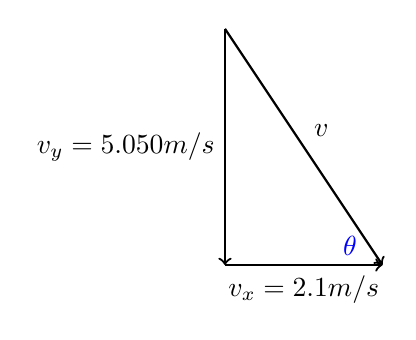
\begin{tikzpicture}
		% Draw the vertical side (v_x)
		\draw[->, thick] (0,0) -- (0,-3) node[midway, left] {$v_y = \SI{5.050}{m/s}$};
		
		% Draw the horizontal side (v_y)
		\draw[->, thick] (0,-3) -- (2,-3) node[midway, below] {$v_x = \SI{2.1}{m/s}$};
		
		% Draw the hypotenuse (v)
		\draw[->, thick] (0,0) -- (2,-3) node[midway, above right] {$v$};
		
		\node at (1.8,-3) [above left,blue] {$\theta$};
		
	\end{tikzpicture}

		Using the pythagorean theorum, we find:
			\begin{equation*}
			v = \sqrt{v_x^2 + v_y^2} = \sqrt{(\SI{2.1}{m/s})^2+(\SI{5.050}{m/s})^2} \approx \SI{5.470}{m/s}
		\end{equation*}
	
	\item The angle of impact is marked as \color{blue} $\theta$ \color{black} in the diagram for part 3.  We can find the angle of impact by using trigonometry.  Using tangent yields:
	
			\begin{equation*}
	\tan {\theta} = \frac{opp}{adj} 
	\end{equation*}

	\begin{equation*}
	\theta = \tan^{-1} (\frac{opp}{adj}) = \tan^{-1} (\frac{v_y}{v_x}) = \tan^{-1} (\frac{\SI{5.050}{m/s}}{\SI{2.1}{m/s}}) \approx 67.420 \degree
	\end{equation*}

		
	\end{enumerate}

	
\end{mdframed}	
	
	
	
	
	
	\subsection{Projectiles Launched at an Arbitrary Angle}
	\index{Projectiles, Launched at an Arbitrary Angle}
	\subsubsection{Projectiles Launched at an Arbitrary Angle on Level Ground}
	\subsubsection{Projectiles Launched at an Arbitrary Angle on Uneven Ground}
	\subsubsection{Projectiles Launched at an Arbitrary Angle Near a Mountain or Hill}
		
		


	



\chapter{Newtons Laws}
	\section{Newton's First Law}
	\section{Newton's Second Law}
	\section{Newton's Thrid Law}
	\section{Applications of Newton's Laws}
		\subsection{Friction}
		\subsection{Elevators}
		\subsection{Pulleys}
		


	


	
\chapter{Work and Energy}
	\section{Work}
	
		\begin{mdframed}[backgroundcolor=orange!20!white]
		\begin{equation}
		W = \vec{F}\cdot\vec{d}  
		\label{eqn:work}
		\end{equation}
	\end{mdframed}
	
	\section{Energy}
	\subsection{Kinetic Energy} \index{Kinetic Energy} \label{Kinetic Energy}
		\begin{mdframed}[backgroundcolor=orange!20!white]
		\begin{equation}
		K = \frac{1}{2}mv^2 
		\label{eqn:kineticenergy}
		\end{equation}
	\end{mdframed}
	
	\subsection{Potential energy}
	\subsubsection{Gravitational Potential Energy} \index{Gravitational Potential Energy} \index{Potential Energy, Gravitational}
	
			\begin{mdframed}[backgroundcolor=orange!20!white]
		\begin{equation}
		U_g = mhg
		\label{eqn:gravitationalpotentialenergy}
		\end{equation}
	\end{mdframed}
	
	\subsubsection{Elastic Potential Energy} \index{Elastic Potential Energy} \index{Potential Energy, Elastic}
	
	\index{Potential Energy, Gravitational}
	
		\begin{mdframed}[backgroundcolor=orange!20!white]
		\begin{equation}
		\overrightarrow{F_s} = -k\vec{x}
		\label{eqn:hookeslaw}
		\end{equation}
	\end{mdframed}
	
	
	\begin{mdframed}[backgroundcolor=orange!20!white]
		\begin{equation}
		U_s = \frac{1}{2}kx^2
		\label{eqn:elasticpotentialenergy}
		\end{equation}
	\end{mdframed}

	While all real springs convert mechanical energy into heat when stretching or compressing, the amount of energy lost as heat (a process called hysteresis) is usually negligible.  However, some stretchable objects, such as rubber bands, lose significant amounts of energy as heat.  Thus, equations \ref{eqn:hookeslaw} and \ref{eqn:elasticpotentialenergy} are not applicable to these objects.  
	
	\section{The Work-Energy Theorem}
	The \textit{Work-Energy Theorem} states that doing work on an object causes that object's energy to change by the same amount as the work done.  This means that an object has 8 Joules of energy, and 2 Joules of work is done on the object, the object will have 10 Joules of work at the end of the process.  	While this is often associated with a change in kinetic energy, the energy change associated with work can also be associated with gravitational potential energy, thermal energy, or any other form of energy.  
	
	\section{The Law of Conservation of Energy}
	States that Energy cannot be created or destroyed (this isn't entirely true.  This law will be tweaked in chapter \color{red} INSERT REFERENCE HERE. \color{black}
	
	\section{Springs}
	
		\begin{mdframed}[backgroundcolor=orange!20!white]
		\begin{equation}
		T_p = 2 \pi \sqrt{\frac{m}{k}}
		\label{eqn:springperiod}
		\end{equation}
	\end{mdframed}
	
	\section{Pendulums}
	A pendulum is any weight on the end of an arm that is free to swing back and forth.  You may have seen pendulums in old-fashioned clocks, and the swings at a park also act like a pendulum.  When a pendulum swings at a small angle ($\theta \lessapprox 5 \deg)$, the period of a pendulum is given by:
	
	\begin{mdframed}[backgroundcolor=orange!20!white]
		\begin{equation}
			T_p = 2 \pi \sqrt{\frac{l}{g}}
			\label{eqn:pendulumperiod}
		\end{equation}
	\end{mdframed}
	
	Notice that the period of a pendulum does not depend on the mass of the bob.  The only two variables that affect its period (assuming a small angle) are the length of the arm and gravity.  
	
	
	 
	

		


	



\chapter{Impulse and Momentum}
	\section{Momentum} \label{momentum} \index{Momentum} \index{Momentum, Linear}
	Linear momentum is defined by the following equation:
	\begin{mdframed}[backgroundcolor=orange!20!white]
		\begin{equation}
		\vec{p} \equiv m \vec{v} 
		\label{eqn:momentum}
		\end{equation}
	\end{mdframed}
	 where $\vec{p}$ is momentum, $m$ is mass, and $\vec{v} $ is velocity.  Determining an object's momentum can be extremely useful in solving problems involving collisions or explosions.  
	 
	 \begin{mdframed}[backgroundcolor=blue!10!white]
	 	\begin{center}
	 		
	 		
	 		\textbf{Example \thesection.1}	
	 	\end{center}
	 	
	 	\textbf{Problem: } A 1400 kg car is traveling at 12 m/s.  What is its momentum? 
	 	\vspace{0.1in}
	 	
	 	\textbf{Solution:} 
	 	Begin by drawing a diagram and identifying variables:
	 	
	 	
	 	\begin{equation*}
	 	\vec{p} = m \vec{v} \equiv 1400 kg \times 12 \frac{m}{s} = 16800 \frac{kg\cdot m}{s}
	 	\end{equation*}
	 	
	 \end{mdframed}
	 \vspace{0.1in}
	 You may notice that the units for momentum are $\frac{kg \cdot m} {s}$.  This is read as ``kilogram meters per second,'' and there is no special name for this unit.  
	 
	 
	\section{Impulse} \label{impulse} \index{Impulse}
		When a force is applied to an object for a certain amount of time, an \textit{impulse} is delivered to that object.  Impulse is defined by the following equation:
	\begin{mdframed}[backgroundcolor=orange!20!white]
		\begin{equation}
		\vec{J} \equiv \vec{F} t 
		\label{eqn:Impulse}
		\end{equation}
	\end{mdframed}
	where $\vec{J}$ is impulse, $\vec{F}$ is force, and $t $ is time. 
	
	
	\section{The Impulse-Momentum Theorem}
	\section{The Law of Conservation of Momentum}
	

		


	



\chapter{Circular Motion and Orbits}
	\section{Centripetal Forces and Accelerations}
	\subsection{Centripetal Force} \index{Force, Centripetal}
	We have already learned that an object in motion will continue to move in a straight line, assuming no forces are acting on the object.  In order for an object to move along a circular path, there must therefore be a force acting on the object to keep it from moving in a straight line.  If you whirl a mass on a string around in a circle, tension in the string keeps the mass from continuing to move in a straight line.  As the Moon orbits the Earth, the gravitational attraction between the Moon and the Earth keeps the Moon in its orbit around the Earth.  Any force that keeps an object moving along a circular path is called a \textbf{Centripetal Force} (Centripetal literally translates from Latin as ``center seeking'').  Any centripetal force can be described as:
	
	\begin{mdframed}[backgroundcolor=orange!20!white]
	\begin{equation}
	F_c = \frac{mv^2}{r}
	\label{equation:centripetalforce}
	\end{equation}
		
	\end{mdframed}
	

	The direction of a centripetal force is always toward the center of the circle.  

	
	\subsection{Centripetal Acceleration} \index{Acceleration, Centripetal}
	
	
	
	When an object moves in a circle, even if its speed remains constant, its velocity is constantly changing due to its constant change in direction of motion.  Thus the object must be constantly accelerating in a direction toward the center of the circle.  Using Equation \ref{equation:centripetalforce} and Newton's Second Law, it is possible to prove that centripetal acceleration is given by:			
	\begin{mdframed}[backgroundcolor=orange!20!white]
	\begin{equation}
	a_c = \frac{v^2}{r}
	\end{equation}
	\end{mdframed}
	Just as Centripetal force is always directed toward the center of the circle, centripetal acceleration is also always directed toward the center of the circle.  
	
	
	\begin{mdframed}[backgroundcolor=blue!10!white]
		\begin{center}
			\textbf{Example \thesubsection}
		\end{center}
		\textbf{Problem:} A children's toy consists of a 0.5kg ball attached to the end of a light 0.3 meter rope.  A child grabs the toy from the end of the rope and swings the ball around in a circle above his head.  What is the tension in the rope? 
		
		\vspace{0.1in}
		
		\textbf{Solution:}
		
		\end{mdframed}
	
	
	\section{Kepler's Laws of Planetary Motion}
	\subsection{Kepler's First Law}
	\subsection{Kepler's Second Law}
	\subsection{Kepler's Third Law}
	
	
	
	
	
	\section{Newton's Law of Universal Gravitation}
	
	\section{Orbital Motion}
	

		


	


		
\chapter{Rotational Mechanics}
	\section{Angular Velocity and Acceleration}
	An object that is spinning can be described using angular velocity and angular acceleration.  Angular velocity is a way of expressing how much an object rotates in a given time.  It could be measured in Rotations per Minute (rpms), Degrees per hour, or any other measurement of an angle divided by any measurement of time.  However, it is advantageous to use Radians per Second.
	
	  Just like velocity measures how fast an object is moving in a line, angular velocity measures how fast an object is rotating.    Average angular velocity is given by the following equation:
	  	\begin{mdframed}[backgroundcolor=orange!20!white]
	  \begin{equation}
		\vec{\omega}_{avg} = \frac{\Delta \vec{\theta}}{\Delta t}
	  \end{equation}
	\end{mdframed}
	and instantaneous angular velocity is given by: 
	  	\begin{mdframed}[backgroundcolor=orange!20!white]
	\begin{equation}
	\vec{\omega} = \frac{d \vec{\theta}}{d t}
	\end{equation}
\end{mdframed}


	\section{Angular Kinematics}
	
	Using the definitions of angular velocity and angular acceleration and a little calculus (or a lot of algebra) we can prove the following four equations:
	
	\begin{mdframed}[backgroundcolor=orange!20!white]
		\begin{center}
			\textbf{The Angular Kinematic Equations}
		\end{center}
		\begin{multicols}{2}
			\begin{equation}
				\vec{\theta} = \frac{\overrightarrow{\omega_f} + \overrightarrow{\omega_i}}{2}  t
				\label{equation:akinematic1}
			\end{equation}
			
			\begin{equation}
				\overrightarrow{\omega_f} = \overrightarrow{\omega_i} + \vec{\alpha} t
				\label{equation:akinematic2}
			\end{equation}	
			
			\begin{equation}
				\vec{\theta} = \overrightarrow{\omega_i} t + \frac{1}{2}\vec{\alpha}{t}^2
				\label{equation:akinematic3}
			\end{equation}
			
			\begin{equation}
				\overrightarrow{\omega_f}^2 = \overrightarrow{\omega_i}^2 + 2\vec{\alpha}\vec{\theta}
				\label{equation:akinematic4}
			\end{equation}
			
			
			
		\end{multicols}
	\end{mdframed}
	
	You may notice that the form of the angular kinematic equations is equivalent to the form of the original, linear kinematic equations introduced in \cref{kinematicequations}. This means that all the intuition and skills developed previously are still valid.   
	
	

	\section{Moment of Inertia}
	\index{Moment of Inertia} \index{Inertia, Moment of} \index{rotational inertia}
	The \textbf{Moment of Inertia} (sometimes called \textbf{rotational inertia}), symbolized $I$, of an object can be thought of as the rotational equivalent of mass.  An object of lesser mass will accelerate more than an object of greater mass when the same amount of force is applied.  Likewise, an object with a smaller moment of inertia will tend to have a greater angular acceleration than an object with a greater moment of inertia when the same forces are applied to the objects.  
	
	The moment of inertia of an object depends both on the mass of the object and the way in which the mass is distributed.  Some common moments of inertia can be found in the attached table.  
	
	\begin{longtable}{|c c|c c |}
		\hline
		Solid Sphere & $I=\frac{2}{5}mr^2$ & Hollow Sphere & $I = \frac{2}{3} m r^2 $  \\	
		\hline
		
	\end{longtable}
	
	
	
	\section{Torque}
	\index{Torque}
	\textbf{Torque} is the rotational equivalent to force.  That is, it is a force that is applied to an object somewhere other than the center of mass, causing the object to rotate.  
	
	
		\begin{mdframed}[backgroundcolor=orange!20!white]
		\begin{equation}
			\vec{\tau} = \vec{r} \times \vec{F}
			\label{equation:torque}
		\end{equation}
	\end{mdframed}
	
	
	You may note that the two vectors are multiplied as a cross product.  The magnitude of the torque is given by:
	
		\begin{mdframed}[backgroundcolor=orange!20!white]
		\begin{equation}
			|\vec{\tau}| = r \cdot F \cdot sin (\theta)
			\label{equation:torquemagnitude}
		\end{equation}
	\end{mdframed}
	
	and the direction is given by the 1st Right Hand Rule (see \cref{RHR1}).
	
	\begin{mdframed}[backgroundcolor=blue!10!white]
		\begin{center}
			
			
			\textbf{Example \thesection.1}	
		\end{center}
		\vspace{0.1in}
		\textbf{Problem:} A force of 10N acts tangentially to the right at the top of a wheel for radius r=0.1 m.  What is the torque exerted on the wheel and in what direction? 
		
		\vspace{0.1in}
		
		\textbf{Solution:} 
		Begin by drawing the diagram:
		\vspace{0.1in}
		
	%	\includegraphics{"./Chapters/Ch09-RotationalMechanics/wheel.png"}
		\vspace{0.1in}
		
		We can use Equation \ref{equation:torquemagnitude} to determine the torque:
		\begin{equation*}
			|\vec{\tau}| = r \cdot F \cdot sin (\theta) = 0.1 \si{m} \cdot 10 \si{N} \cdot \sin( 90 \degree) = \boxed{1 \si{m \times N}}
		\end{equation*}
		
		The direction of the torque is given by the 1st right hand rule.  Your index finger points along the direction of $\vec{r}$.  Your middle finger bends 90 degrees and aligns with $\vec F$.  Your thumb shows the resulting direction of the torque: \textbf{into the page.}
		
	\end{mdframed}
	
	
	
	
	
	
	
	\subsection{Newton's Laws in a Rotational Setting}
	\index{Newton's Laws, Rotational}
	
	\subsubsection{Newton's First Law for Rotation}
	Objects in uniform rotational motion will remain in uniform rotational motion and objects at rotational rest will remain at rotational rest until acted upon by an external, unbalanced torque.  
	
	\subsubsection{Newton's Second Law for Rotation}
			\begin{mdframed}[backgroundcolor=orange!20!white]
		\begin{equation}
			\vec{\tau} = I \cdot \vec{\alpha}
			\label{equation:newtonssecondrotational}
		\end{equation}
	\end{mdframed}
	
	\subsubsection{Newton's Third Law for Rotation}
	For every torque, there is an equal opposite torque.
	
	
	\section{Angular Kinetic Energy}
	\index{Angular Kinetic Energy}
	\index{Kinetic Energy, Angular}
	
	\textbf{Angular Kinetic Energy}, sometimes called rotational kinetic energy, is energy of rotational motion.  An object that is only rotating - like a fan - has angular kinetic energy only.  An object that is rolling - like the wheel of a car - has both translational kinetic energy (found using $k = \frac{1}{2}mv^2$ ) and angular kinetic energy, found using:
	
				\begin{mdframed}[backgroundcolor=orange!20!white]
		\begin{equation}
			K = \frac{1}{2}I\omega^2
			\label{equation:rotationalkineticenergy}
		\end{equation}
	\end{mdframed}
	
	\newpage
	\section{Angular Momentum} \label{angularmomentum} \index{Angular Momentum}
	\subsection{The Definition of Angular Momentum}
	Angular momentum can be calculated using the formula: 
	 	\begin{mdframed}[backgroundcolor=orange!20!white]
		\begin{equation}
		\vec{L} = I \vec{\omega}
		\label{equation:angularmomentum}
				\end{equation}
	\end{mdframed}
where $\vec{L}$ is angular momentum, $I$ is the object's moment of Inertia and $\vec{\omega}$ is the object's angular velocity.  The SI units for angular momentum are  $\frac{kg m^2} {s} $.


\begin{mdframed}[backgroundcolor=blue!10!white]
	\begin{center}
		
		
		\textbf{Example \thesection.1}	
	\end{center}
	\vspace{0.1in}
	\textbf{Problem:} A bicycle wheel has a mass of 0.3 kg, and can be thought of as a thin ring with a radius of 0.33m. When the wheel is turning at a rate of 2 rotations per second, what its its angular momentum?
	\vspace{0.1in}
	
	\textbf{Solution:} 
	Begin by converting the angular velocity $\omega$ to appropriate units:
	\begin{equation*}
	\vec{\omega} = 2 \frac{rotations}{s} = 4\pi \frac{rad}{s}
	\end{equation*}
	
	Then calculate the moment of inertia.  Using the formula for a thin ring: 
	\begin{equation*}
	I  = mr^2 = 0.3 kg  (0.33m)^2 \approx 0.033 kg m^2
	\end{equation*}
	Finally, use equation \ref{equation:angularmomentum} to find the angular momentum. 
	
	\begin{equation*}
	\vec{L}  =  I \vec{\omega} = 0.011 kg m^2 \cdot 4\pi \frac{rad}{s} \approx \boxed{0.411 \frac{kg m^2}{s}}
	\end{equation*}
	
	
	
\end{mdframed}


	\subsection{Conservation of Angular Momentum}
 Just like linear momentum\footnote{see momentum in \cref{angularmomentum}}, angular momentum is a quantity that is conserved.  Thus, whatever angular momentum a closed system has in its initial state will be equal to the angular momentum the system has in its final state.  
 
 The classic example of the Law of Conservation of Momentum is an ice skater who enters a spin.  By changing the positioning of his or her arms and legs, an ice skater can change their moment of inertia.  When they bring their arms and legs closer to their axis of rotation, their moment of inertia decreases.  Since angular momentum is conserved, their angular velocity must increase as their moment of inertia decreases, and thus the ice skater is able to spin very fast. 
 
	
	

		


	


		







\appendix

\appendixpage
\noappendicestocpagenum
\addappheadtotoc





\chapter{Math Skills}

\section{Scientific Notation}


	\begin{itemize}
		\item Scientific Notation always has three parts: the \textit{coefficient}, the \textit{base}, and the \textit{exponent}:
		\begin{center}
			\color{blue} Coefficient $\rightarrow \color{black} 6.022 \times 10^{23 \color{red}\leftarrow}$ \textsuperscript{\color{red}Exponent} \color{black}
			
			\hspace{.7in} \color{orange}$\uparrow$
			
			\hspace{.7in} Base \color{black}
		\end{center}
		\item In scientific notation the \color{orange} base \color{black}is always 10. 
		\item A negative in front of the  \color{blue} coefficient \color{black} means the whole number is negative. 
		\item  A negative \color{red} exponent \color{black} means the number is very small (close to zero). \color{black}
		\item  The \color{red} exponent \color{black} counts how many places the decimal moved, NOT the number of zeroes.	
		\item When comparing numbers in scientific notation, look at (in order): 
		\begin{enumerate}
			\item  Negatives in front of the \color{blue} coefficient. \color{black}
			\item \color{red}Exponents \color{black}
			\item \color{blue}Coefficients \color{black}
		\end{enumerate}
		
		\item To multiply, multiply coeffients, then ADD exponents.
		\item To divide, divide coefficients, then SUBTRACT exponents.
		\item To raise to a power, raise the coefficient to the power, then MULTIPLY exponents.
		\item To enter scientific notation on most calculators use the ``EE" key. $6.022 \times 10^{23}$ is entered as 6.022\scriptsize E\normalsize23.  Calculator notation should \underline{\textbf{never}} be handwritten. 
		\item Metric Prefixes are really just scientific notation:
		\begin{center}
			\begin{tabular}{|c|c|c|}
				\hline
				Prefix & Letter & Power of 10 \\
				\hline
				nano & n &  $ \times 10^{-9}$ \\
				\hline
				micro & $\mu$ &  $ \times 10^{-6}$ \\
				\hline
				milli & m & $ \times 10^{-3}$ \\
				\hline
				centi & c & $ \times 10^{-2}$ \\
				\hline
				deci & d & $ \times 10^{-1}$ \\
				\hline
				Deka & D & $ \times 10^{1}$ \\
				\hline
				Hecto & H & $ \times 10^{2}$ \\
				\hline
				Kilo & k & $ \times 10^{3}$ \\
				\hline
				Mega & M & $ \times 10^{6}$ \\
				\hline
				Giga & G & $ \times 10^{9}$ \\
				\hline
				
			\end{tabular}	
		\end{center}
		
		
	\end{itemize}
\newpage

\section{Algebra}
To study physics, you should have some knowledge of algebra. Though this appendix is too small to include all algebraic techniques, there are some things that are repeated often in physics. These commonly recurring algebraic themes are highlighted here.

\subsection{Solve for a Variable}

Solving for a variable is one of the most fundamental skills in algebra and physics. Whether you're isolating a variable to find a force, velocity, or time, this process involves rearranging equations using inverse operations.



\begin{mdframed}[backgroundcolor=blue!10!white]
	\begin{center}
		
		
		\textbf{Example \thesection.1}	
	\end{center}
	
	\textbf{Problem:} Solve the Equation \color{blue}$2x+3 = 12x +1$  \color{black} for \color{blue}$x$\color{black}.
	\vspace{0.1in}
	
	\textbf{Solution:} To solve this equation, we begin by combining like terms.  Terms involving \color{blue}$x $ \color{black} should be moved to one side, while terms involving only numbers are moved to the other.  
	\color{blue}
	
	\begin{equation*}
		2x + 3 = 12 x +1
	\end{equation*}
	\begin{equation*}
	-10x +3  = 1
\end{equation*}
	\begin{equation*}
	-10x = -2
\end{equation*}
\color{black}


Now, dividing by -10 gives: 
	\color{blue}
	\begin{equation*}
	x = 5
\end{equation*}	
	\color{black}
\end{mdframed}
\newpage

\subsubsection{Solve for a Variable in the Denominator of a Fraction}

Sometimes, the variable you're solving for appears in the denominator. This can often be confusing at first, but the trick is to eliminate the fraction by multiplying both sides by the denominator.

\begin{mdframed}[backgroundcolor=blue!10!white]
	\begin{center}
	
	
	\textbf{Example \thesection.1.2}	
\end{center}

\textbf{Problem:} Solve for \( R \) in the equation:

	\begin{equation*}
			V = \frac{I}{R}
	\end{equation*}

	


\textbf{Solution:} Multiply both sides by \( R \) to eliminate the denominator:
\[
V \cdot R = I
\]
Then divide both sides by \( V \) to isolate \( R \):
\[
R = \frac{I}{V}
\]

\end{mdframed}

\subsubsection{Solve for a Variable using the Quadratic Formula} \index{Quadratic Forumula}

In some physics problems, especially those involving kinematics or energy, you might encounter equations that take the form of a quadratic:

\[
ax^2 + bx + c = 0
\]

The solution is given by the quadratic formula:
\[
x = \frac{-b \pm \sqrt{b^2 - 4ac}}{2a}
\]

\begin{mdframed}[backgroundcolor=blue!10!white]
	\begin{center}
		
		
		\textbf{Example \thesection.1.3}	
	\end{center}
	
	\textbf{Problem:}
	Solve for \( t \):
	\[
	0 = 5t^2 - 20t + 15
	\]


\textbf{Solution:} Identify \( a = 5 \), \( b = -20 \), and \( c = 15 \). Plug into the quadratic formula:

\[
t = \frac{-(-20) \pm \sqrt{(-20)^2 - 4(5)(15)}}{2(5)} = \frac{20 \pm \sqrt{400 - 300}}{10} = \frac{20 \pm \sqrt{100}}{10}
\]

\[
t = \frac{20 \pm 10}{10} = 3 \text{ or } 1
\]

It should be noted that negative answers can arise in physics, and negatives often indicate direction.  However, context tells you which solutions are meaningful.  While a negative velocity may just mean an object is traveling opposite the expected direction, a negative time is likely meaningless.

\end{mdframed}
\newpage

\subsection{Solve a System of Equations}

Many physics problems involve more than one equation and variable. These systems can be solved using several algebraic techniques.

\subsubsection{Solve a System of Equations by Combination}

Also called the addition or elimination method, this approach involves adding or subtracting equations to eliminate one variable.  This is particularly useful when coefficients are opposites or can easily be made opposites.

\begin{mdframed}[backgroundcolor=blue!10!white]
	\begin{center}
		
		
		\textbf{Example \thesection.1.4}	
	\end{center}
	
	\textbf{Problem:}
	Solve the system:
	\[
	\begin{aligned}
		2x + 3y &= 12 \\
		4x - 3y &= 6
	\end{aligned}
	\]


\textbf{Solution:} Add the equations to eliminate \( y \):
	\[
\begin{aligned}
	2x + 3y &= 12 \\
	+  \hspace{0.1in} 4x - 3y &= 6\\
	\hline
	6x \hspace{0.3in} &= 18 \\
	x&=3
\end{aligned}
\]

Substitute \( x = 3 \) into the first equation:
\[
2(3) + 3y = 12 \Rightarrow 6 + 3y = 12 \Rightarrow y = 2
\]


\end{mdframed}

\newpage
\subsubsection{Solve a System of Equations by Substitution}

This method is ideal when one of the equations is already solved for one variable, or can easily be rearranged to do so. 

\begin{mdframed}[backgroundcolor=blue!10!white]
	\begin{center}
		
		
		\textbf{Example \thesection.1.5}	
	\end{center}
	
	\textbf{Problem:}
	Solve the system:
	\[
	\begin{aligned}
		y &= 2x + 1 \\
		3x + y &= 16
	\end{aligned}
	\]


\textbf{Solution:} Substitute the expression for \( y \) into the second equation:
\begin{equation*}
3x + (2x + 1) = 16 	
\end{equation*}
\begin{equation*}
	 5x + 1 = 16 
\end{equation*}
\begin{equation*}
	 5x = 15
	 \end{equation*}
 \begin{equation*}
 	x = 3
 \end{equation*} 

Now substitute back to find \( y \):
\[
y = 2(3) + 1 = 7
\]

\end{mdframed}

\newpage
\subsubsection{Solve a System of Equations using Matrices}

Matrices are useful for solving larger systems of equations, especially in physics problems involving circuits or forces in multiple directions.  If you have three or more variables an equal number of equations, using a matrix to solve the problem keeps your work organized as well.  You may use any of the following operations:
\begin{itemize}
	\item Multiply or divide any row by a constant.
	\item Add two rows together, and replace either row with the result.
	\item Swap the order of rows.
\end{itemize}


\begin{mdframed}[backgroundcolor=blue!10!white]
	\begin{center}
		
		
		\textbf{Example \thesection.1.5}	
	\end{center}
	
	\textbf{Problem:}

	Solve the system using matrices:
\begin{equation*}
	\begin{aligned}
	2x + 3y + z &= 8 \\
	x + y - z &= 1 \\
	3x + 2y + z &= 15
\end{aligned}
\end{equation*}


\textbf{Solution:} Begin by writing the equations as an augmented matrix: 
\vspace{-0.2in}

	\begin{equation*}
\begin{bmatrix}
	2 & 3 & 1 & 8 \\
	1 & 1 & -1 & 1\\
	3 & 2 & 1 & 15 
\end{bmatrix} 		
	\end{equation*}

First, we can multiply the 2nd row by -2.

	\begin{equation*}
		R_2 = -2 R_2 \longrightarrow
	\begin{bmatrix}
		2 & 3 & 1 & 8 \\
		-2 & -2 & 2 & -2\\
		3 & 2 & 1 & 15 
	\end{bmatrix} 		
\end{equation*}

Now we add Row 1 to Row 2:

\begin{equation*}
	R_2 = R_1 + R_2 \longrightarrow
	\begin{bmatrix}
		2 & 3 & 1 & 8 \\
		0 & 1 & 3 & 6\\
		3 & 2 & 1 & 15 
	\end{bmatrix} 		
\end{equation*}

Next, we multiply Row 1 by 3 and row 3 by -2:

\begin{equation*}
	\begin{aligned}
		R_1 &= 3 R_1 \\
		R_3 &= -2 R_3
	\end{aligned}
	\longrightarrow
	\begin{bmatrix}
		6 & 9 & 3 & 24 \\
		0 & 1 & 3 & 6\\
		-6 & -4 & -2 & -30 
	\end{bmatrix} 		
\end{equation*}

Now we can add Row 1 to Row 3:
\begin{equation*}
	R_3 = R_1 + R_3
	\longrightarrow
\begin{bmatrix}
	6 & 9 & 3 & 24 \\
	0 & 1 & 3 & 6\\
	0 & 5 & 1 & -6 
\end{bmatrix} 	
\end{equation*}

Multiplying row 2 by -5 gives:
\begin{equation*}
	R_2 = -5R_2
	\longrightarrow
	\begin{bmatrix}
		6 & 9 & 3 & 24 \\
		0 & -5 & -15 & -30\\
		0 & 5 & 1 & -6 
	\end{bmatrix} 	
\end{equation*}

Adding Row 2 and row 3 yields:
\begin{equation*}
	R_3 = R_2 + R_3
	\longrightarrow
	\begin{bmatrix}
		6 & 9 & 3 & 24 \\
		0 & -5 & -15 & -30\\
		0 & 0 & -14 & -36 
	\end{bmatrix} 	
\end{equation*}

Now we can divide Row 3 by -14:

\begin{equation*}
	R_3 = \frac{R_3}{-14}
	\longrightarrow
	\begin{bmatrix}
		6 & 9 & 3 & 24 \\
		0 & -5 & -15 & -30\\
		0 & 0 & 1 & \frac{18}{7} 
	\end{bmatrix} 	
\end{equation*}

This means that $z = \frac{18}{7}$.  Continuing to solve the problem, we can multiply row 3 by 15 and add it to row 2 to to get: 

\begin{equation*}
	R_2 = R_2 + 15 R_3  
	\longrightarrow
	\begin{bmatrix}
		6 & 9 & 3 & 24 \\
		0 & -5 & 0 & \frac{60}{7}\\
		0 & 0 & 1 & \frac{18}{7} 
	\end{bmatrix} 	
\end{equation*}

Now, divide row 2 by -5:

\begin{equation*}
	R_2 = \frac{R_2}{5}   
	\longrightarrow
	\begin{bmatrix}
		6 & 9 & 3 & 24 \\
		0 & 1 & 0 & \frac{-12}{7}\\
		0 & 0 & 1 & \frac{18}{7} 
	\end{bmatrix} 	
\end{equation*}

Which means we now know $y = \frac{-12}{7}$.  We can now use row 2 and row 3 to eliminate variables in row 1:  

\begin{equation*}
	R_1 = R1 + (-9 R_2) + (-3 R_3)  
	\longrightarrow
	\begin{bmatrix}
		6 & 0 & 0 & \frac{222}{7} \\
		0 & 1 & 0 & \frac{-12}{7}\\
		0 & 0 & 1 & \frac{18}{7} 
	\end{bmatrix} 	
\end{equation*}

Finally, dividing Row 1 by 6 gives: 
\begin{equation*}
	R_1 = \frac{R_1}{6}
	\longrightarrow
	\begin{bmatrix}
		1 & 0 & 0 & \frac{37}{7} \\
		0 & 1 & 0 & \frac{-12}{7}\\
		0 & 0 & 1 & \frac{18}{7} 
	\end{bmatrix} 	
\end{equation*}


\end{mdframed}



\newpage
\section{Proportional Reasoning}
\subsection{Proportional Reasoning}

Proportional reasoning is a powerful tool in physics. Often, you don’t need to plug in numbers to figure out how a change in one variable affects another. You only need to understand how variables are related in a formula.

\textbf{The idea:} If a formula contains multiple variables, and you know how one variable changes, you can predict how the output will change—assuming all other variables stay constant or have known changes.


	The force of gravity between two masses is given by:
	\[
	F = G \frac{m_1 m_2}{r^2}
	\]
	A planet has twice Earth’s mass and three times Earth’s radius. If the gravitational force on a mass on Earth is \( F_E \), what is the gravitational force on the same mass on the new planet, in terms of \( F_E \)?


\textbf{Solution:} Let Earth have mass \( M \), and radius \( R \), so:
\[
F_E = G \frac{m M}{R^2}
\]

On the new planet:
\[
F' = G \frac{m (2M)}{(3R)^2} = G \frac{2mM}{9R^2} = \frac{2}{9} F_E
\]

\textbf{Answer:} \( \frac{2}{9} F_E \)

\textbf{Comment:} The trick is to substitute the new values into the formula and simplify. Don’t calculate anything you don’t need.

\vspace{1em}

	The period \( T \) of a pendulum is given by:
	\[
	T = 2\pi \sqrt{\frac{L}{g}}
	\]
	If the length \( L \) of a pendulum is quadrupled, by what factor does the period \( T \) change?


\textbf{Solution:}
\[
T' = 2\pi \sqrt{\frac{4L}{g}} = 2\pi \cdot 2\sqrt{\frac{L}{g}} = 2T
\]

\textbf{Answer:} The period doubles.

\textbf{Comment:} When a variable is inside a square root, its effect is weaker. Quadrupling \( L \) only doubles \( T \).

\vspace{1em}

	The kinetic energy of an object is:
	\[
	K = \frac{1}{2}mv^2
	\]
	If the velocity of the object triples, how does its kinetic energy change?


\textbf{Solution:}
\[
K' = \frac{1}{2} m (3v)^2 = \frac{1}{2} m \cdot 9v^2 = 9K
\]

\textbf{Answer:} The kinetic energy increases by a factor of 9.

\textbf{Comment:} Pay attention to exponents—tripling \( v \) squares the effect in \( v^2 \).

\vspace{1em}

	The electric force between two charges is given by:
	\[
	F = k \frac{q_1 q_2}{r^2}
	\]
	If both charges are doubled and the distance is halved, what happens to the electric force?


\textbf{Solution:}
\[
F' = k \frac{(2q_1)(2q_2)}{(r/2)^2} = k \frac{4q_1 q_2}{r^2/4} = k \frac{4q_1 q_2 \cdot 4}{r^2} = 16F
\]

\textbf{Answer:} The force increases by a factor of 16.

\textbf{Comment:} Changing more than one variable? Just multiply each effect together.

\vspace{1em}

	The pressure at the bottom of a fluid is given by:
	\[
	P = \rho g h
	\]
	If the height of the fluid is doubled and the fluid is twice as dense, what happens to the pressure?


\textbf{Solution:}
\[
P' = (2\rho) g (2h) = 4 \rho g h = 4P
\]

\textbf{Answer:} The pressure increases by a factor of 4.

\textbf{Comment:} Linear relationships like this are easy to reason through—just multiply the scaling factors.


\newpage
\section{Trigonometry}

\newpage
\section {Radians and Arc Length}
\subsection{Radians} \index{Radians}

Just like there are many different units that measure distance (meters, feet, inches, miles, furlongs, etc.), there are also different ways of measuring angles.  You are probably already familiar with degrees. A right angle is $90 \degree$, and a full circle is $360 \degree$.  When calculating arc length or using the angular kinematic equations, the standard units for angles are \textit{radians}\footnote{It should be noted that strictly speaking, radians are not a unit; since the definition of a radian has to do with a ratio, all numbers with radians as the unit are actually unitless.}  There are $2 \pi$ radians in a complete circle, so,

	\begin{mdframed}[backgroundcolor=green!20!white]
	\begin{equation*}
		360 \degree = 2 \pi \, \si{radians}
		\label{conversion:radiandegree}
	\end{equation*}
\end{mdframed}	

This equation can be used to convert an angle from radians to degrees or vice-versa.  

 \begin{mdframed}[backgroundcolor=blue!10!white]
	\begin{center}	
		\textbf{Example \thesection.1}	
	\end{center}
	
	\textbf{Problem:} An angle measures $34 \degree$.  What is this angle in radians? 
	
	\vspace{0.2 in} 
	\textbf{Solution}: Begin by creating a conversion factor.  In this case, since we have degrees and want radians, we create a fraction with $2\pi$ radians on top of the fraction, and $360\degree$ on the bottom.  Multiplying by this fraction gives:
	
\begin{equation*}
	34 \degree \times \frac{2 \pi \, \si{rad}}{360 \degree} = \frac{17 \pi}{90}\si{rad} \approx 0.593 \, \si{rad}  
\end{equation*}
	
	It should be noted that the fraction $\frac{2 \pi \, \si{rad}}{360 \degree}$ can easily be reduced to $\frac{ \pi \, \si{rad}}{180 \degree}$ .  Using this as your conversion factor will yield the same results.  It is also often easier and more accurate to leave measurements involving radians in terms of $\pi$.  
	
\end{mdframed}
   
   
    \begin{mdframed}[backgroundcolor=blue!10!white]
   	\begin{center}	
   		\textbf{Example \thesection.2}	
   	\end{center}
   	
   	\textbf{Problem:} An angle measures $\frac{\pi}{2} \si{rad}$.  What is this angle in degrees? 
   	
   	\vspace{0.2 in} 
   	\textbf{Solution}: Again, we begin by creating a conversion factor.  Because we have a measurement in radians and are asked to find degrees, we create a fraction with $360\degree$ on top of the fraction, and  $2\pi$ radians on the bottom:
   	
   	\begin{equation*}
   		\frac{\pi}{2}  \times \frac{360 \degree}{2 \pi \, \si{rad}} = 90 \degree
   	\end{equation*}
 
   	
   \end{mdframed}

\newpage
   \subsection{Arc Length} \index{Arc Length}
   
   The distance along the circumference of a circle that corresponds to an internal angle of the circle is called \textit{Arc Length}.  Though arc-length is a measurement of length, the symbol used for Arc Length is $s$. 
 \begin{figure}[h]
 	  \begin{center}
   	 	\begin{tikzpicture}
   		% the origin
   		\coordinate (O) at (0,0);
   		% the circle and the dot at the origin
   		\draw (O) node[circle,inner sep=1.5pt,fill] {} circle [radius=3cm];
   		% the ``\theta'' arc
   		\draw 
   		(3 cm,0) coordinate (xcoord) -- 
   		node[midway,below] {$r$} (O) -- 
   		(60:3 cm) coordinate (slcoord)
   		pic [draw,->,angle radius=1cm,"$\theta$"] {angle = xcoord--O--slcoord};
   		% the outer ``s'' arc
   		\draw[|-|]
   		(3 cm +10pt,0)
   		arc[start angle=0,end angle=60,radius=3cm+10pt]
   		node[midway,fill=white] {$s$};
   	\end{tikzpicture}
   \end{center}
 \caption{The relationship between arc-length, radius, and angle}
 \end{figure}
   	
  
   	

   
   
   
   
   
   
   
   
   
    Arc Length can be found using the following equation:
   
   	\begin{mdframed}[backgroundcolor=orange!20!white]
   	
   	\begin{equation}
   		s = r \theta
   		\label{equation:arclength}
   	\end{equation}
   \end{mdframed}
where $r$ is the radius of the circle and $\theta$ is the internal angle, measured in radians. Additionally, while meters are the proper SI units for these measurements, this formula will work with any units of length as long as both arc-length, $s$, and radius, $r$ are measured using the same units.  




\newpage

  \begin{mdframed}[backgroundcolor=blue!10!white]
	\begin{center}	
		\textbf{Example \thesection.2}	
	\end{center}
	
	\textbf{Problem:} Find the arc length of $30\degree$ of a circle with a radius of 0.2 meters.  
	 
	
	\vspace{0.2 in} 
	\textbf{Solution}: Begin by drawing a diagram:
	
	
	 	  \begin{center}
		\begin{tikzpicture}
			% the origin
			\coordinate (O) at (0,0);
			% the circle and the dot at the origin
			\draw (O) node[circle,inner sep=1.5pt,fill] {} circle [radius=3cm];
			% the ``\theta'' arc
			\draw 
			(3 cm,0) coordinate (xcoord) -- 
			node[midway,below] {$0.2 \si{m}$} (O) -- 
			(30:3 cm) coordinate (slcoord)
			pic [draw,->,angle radius=1.6cm,"$30 \degree$"] {angle = xcoord--O--slcoord};
			% the outer ``s'' arc
			\draw[|-|]
			(3 cm +10pt,0)
			arc[start angle=0,end angle=30,radius=3cm+10pt]
			node[midway,fill=blue!10!white] {$s$};
		\end{tikzpicture}
	\end{center}

	In order to find arc length, we must first convert the angle from degrees to radians:
	\begin{equation*}
	\theta = 30 \degree \times \frac{2 \pi \si{rad}} {360 \degree} = \frac{\pi}{6} \si{rad}
	\end{equation*}
	
	Now, arc length can be found using equation \ref{equation:arclength}.
	\begin{equation*}
		s = r \theta = (0.2 \si{m})(\frac{\pi}{6} \si{rad}) \approx 0.105 \si{m}
	\end{equation*}
	
	
\end{mdframed}
  



\chapter{Reference Tables}
\section{Greek Letters}
\index{GreekLetters}
\section{Physical Constants}
\index{Physical}

		
	\backmatter	
	
\printindex		








\end{document}